\begin{figure}[H]
\center

\includegraphics[scale=1]{kibana.png}
\label{fig:kibana.png}
\end{figure}
\section{Qu'est ce que Kibana}
Kibana est à la fois un front-end à Elasticsearch mais également un outil de présentation
de données puissant. Kibana permet aussi dans une certaine mesure de faire du monitoring.
(avec de grosses guillemets quand même)

Il est principalement codé en angularJS.

C'est l'outil de visualisation officiel d'Elasticsearch, il est assez ergonomique 
et donc plutôt facile d'utilisation. Sa barre de recherche utilise la syntaxe 
search Lite présenté plus dans le chapitre traitant d'Elasticsearch.
Son utilisation pour réaliser des tableaux, dashboard et autre camemberts est assez
aisé une fois les principes de bases assimilés.

\section{Installation de Kibana}
L'installation de Kibana est relativement simple, il suffit de télécharger l'application
compressé à l'adresse sur le site de \url{https://download.elastic.co/kibana/kibana/kibana-4.0.2-linux-x64.tar.gz}{elastic}.
On décompresse, on lance (\ipath{path/bin/kibana}), et c'est parti !
Évidemment, si on execute kibana d'une telle manière il est préferable de le lancer
depuis un tmux ou un screen (ou un quelconque multiplexeur de terminal). Il est 
également facile de réaliser son propre service systemd.

\subsection{Paramétrage}
Afin de pouvoir se connecter à Elasticsearch il faut tout de même renseigner 
\ipath{path/config/kibana.yml} notamment : \emph{port} (par défaut 5601), \emph{host} (ip d'écoute)
et surtout \emph{elasticsearch\_url}.
Dans des circonstances normales c'est tout ce que vous aurez à paramétrer (hors 
SSL \ldots{}).

Il peut arriver dans de rares cas (lorsque Elasticsearch est saturé ou bien lors 
d'une requête particulièrement gourmande) que kibana se ferme car Elasticsearch met
trop de temps à répondre. Il est dans ces cas là, il est fortement conseillé de 
redémarrer l'instance en question, d'étendre sa \emph{HEAP\_SIZE}, ou bien si possible, 
rajouter de la RAM.

Il est possible de modifier le requestTimeout dans \ipath{path/src/lib/waitForEs.js}
C'est pour l'instant la seule façon de faire, d'après une issue github, la prochaine 
mouture de kibana devrait intégrer ce paramètre dans son fichier de configuration.

\section{Utilisation de Kibana}
Dans cette partie nous allons faire une brève présentation (illustré) de Kibana et
de son fonctionnement.

\subsection{Recherche}
\begin{figure}[H]
\center
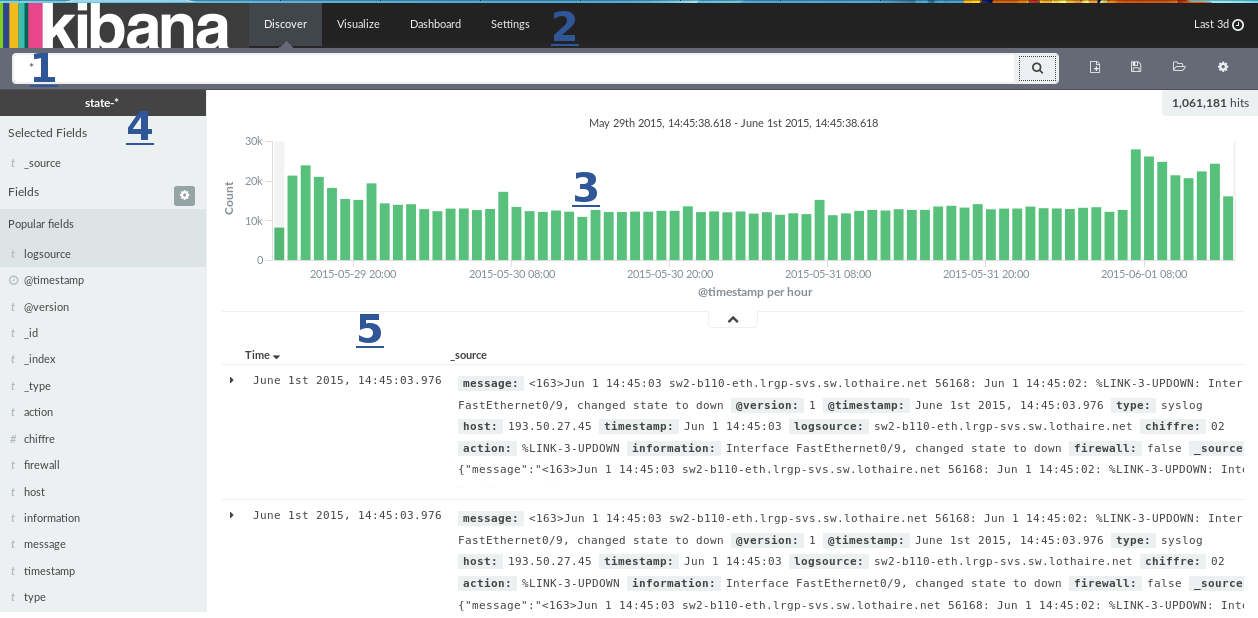
\includegraphics[width=1\textwidth]{kibanatuto/rap/1.png}
\label{fig:kibanatuto1}
\caption{Présentation générale de Kibana}
\end{figure}

Voici la page principale sur laquelle on arrive lorsque l'on se connecte à Kibana
depuis son navigateur.

\begin{enumerate}
    \item La barre de recherche \\(syntaxe SearchLite)
    \item Barre de sélection des \emph{modes} \\(Discover : Recherche, Visualize : Création 
    de Tableaux et autre représentations graphiques, Dashboard : Rassemblement de
    ces présentations, Settings : Paramétrage de certaines options)
    \item Tableau graphique des résultats de recherche
    \item Tableau des champs de l'index
    \item Tableaux des lignes correspondant à la recherche
\end{enumerate}


\begin{figure}[H]
\center
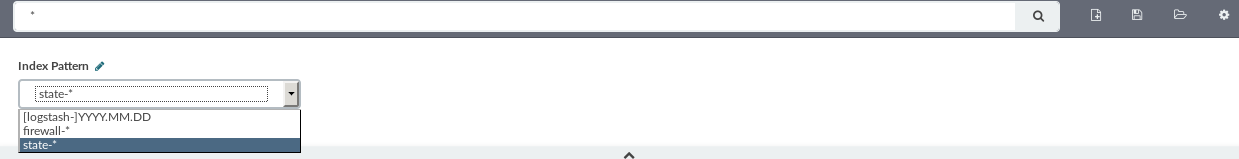
\includegraphics[width=1\textwidth]{kibanatuto/rap/2.png}
\label{fig:kibanatuto2}
\caption{Choisir son index pour une recherche}
\end{figure}
Pour effectuer une recherche, on doit choisir dans quels index, si il est possible 
de réaliser une recherche dans plusieurs index à la fois, il faut dans Kibana que 
ce soit des indexs disposant du même mapping. Typiquement rangés par \ipath{nom-*}.
Pour choisir son index il faut \emph{sélectionner la roue denté à droite de la barre
de recherche}.


\begin{figure}[H]
\center
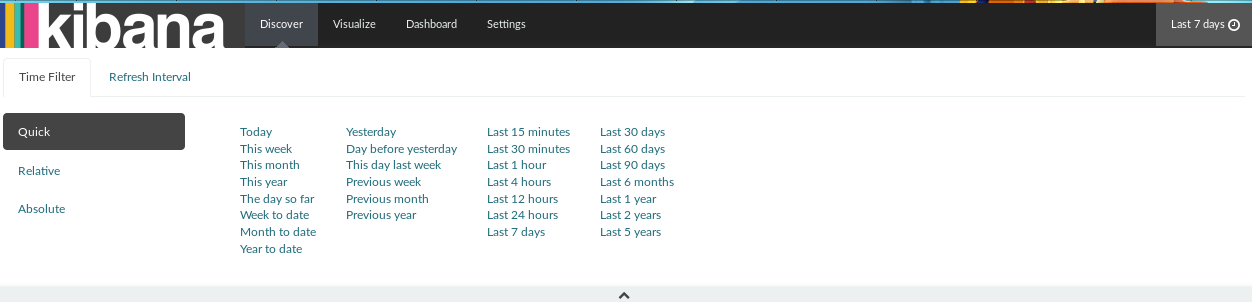
\includegraphics[width=1\textwidth]{kibanatuto/rap/3.png}
\label{fig:kibanatuto3}
\caption{Choisir son intervalle de temps}
\end{figure}
Lorsque l'on effectue une recherche avec Kibana il est possible de choisir de façon
très flexible son intervalle de temps (bouton de temps en haut à droite).
Il est tout d'abord possible de de choisir les possibilités du menu rapide, affichées
dans l'image ci-dessus. Le choix est déjà assez exhaustif, mais il est également 
possible de se positionner relativement par rapport à maintenant. Par exemple rechercher 
parmi les 30 dernières secondes, ou bien les deux derniers mois (de la seconde à 
l'année). Il est également possible de choisir un intervalle de temps absolue, à 
la seconde près.

Enfin il est possible de rafraichir ces données en choisissant un intervalle allant
de 5 secondes à une journée (également désactivable).
\newpage
%\begin{wrapfigure}{l}{0.42\textwidth}
\begin{figure}[H]
\center
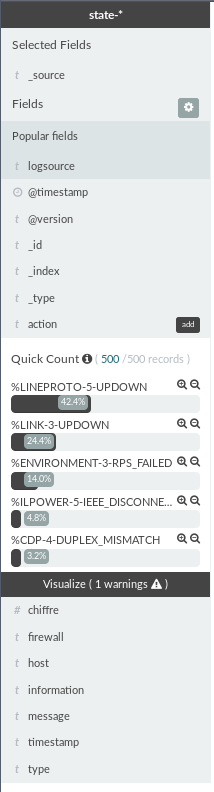
\includegraphics[width=0.4\textwidth,height=0.8\textheight]{kibanatuto/rap/4.png}
\label{fig:kibanatuto4}
\caption{Le tableau des champs}
\end{figure}
%\end{wrapfigure}

Le tableau des champs disponibles dans l'index est très pratique pour rendre plus 
lisible les informations que l'on recherche ainsi que pour obtenir des statistiques 
rapides sur les occurrences des termes les plus communs.

Ce tableau contient tous les champs disponibles dans l'index. Il est possible de
faire de la ségrégation dans les résultats de nos recherches en incluant ou en   
excluant un ou plusieurs termes proposés {\footnotesize\textit{(on peut par exemple exclure le résultat 
le plus courant car on sait un switch défectueux, afin de se concentrer sur les autres
pannes pas encore détectées et donc plus pertinentes)}}. Il suffit pour cela d'appuyer
sur les loupes situées à droite des termes suggérés.


Il est également possible de choisir de ne montrer que \hyperref[fig:kibanatuto6]{la ou les parties que l'on 
estime pertinente} dans le log (en appuyant sur le \hyperref[fig:kibanatuto5]{bouton 
add à droite} de chaque champ) et bien sure de combiner les deux dernières "techniques".
\begin{figure}[H]
\begin{flushright}

\includegraphics[width=0.3\textwidth]{kibanatuto/rap/8.png}
\label{fig:kibanatuto5}
\end{flushright}%
\end{figure}

\begin{figure}[H]
\center
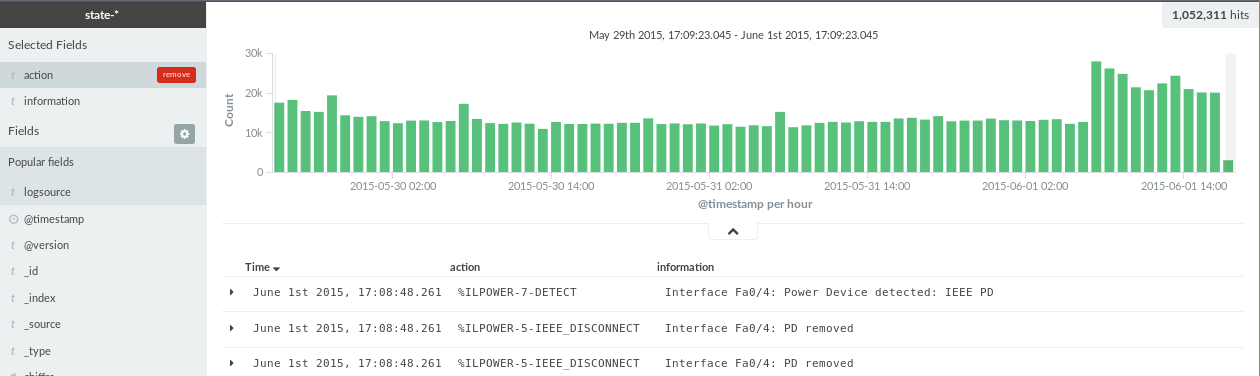
\includegraphics[width=1\textwidth]{kibanatuto/rap/9.png}
\label{fig:kibanatuto6}
\caption{Résultat}
\end{figure}

\subsection{Visualization}
Nous allons maintenant parler de la visualisation des données, il s'agit la encore
que de donner un très bref aperçu des possibilités.

\begin{figure}[H]
\center
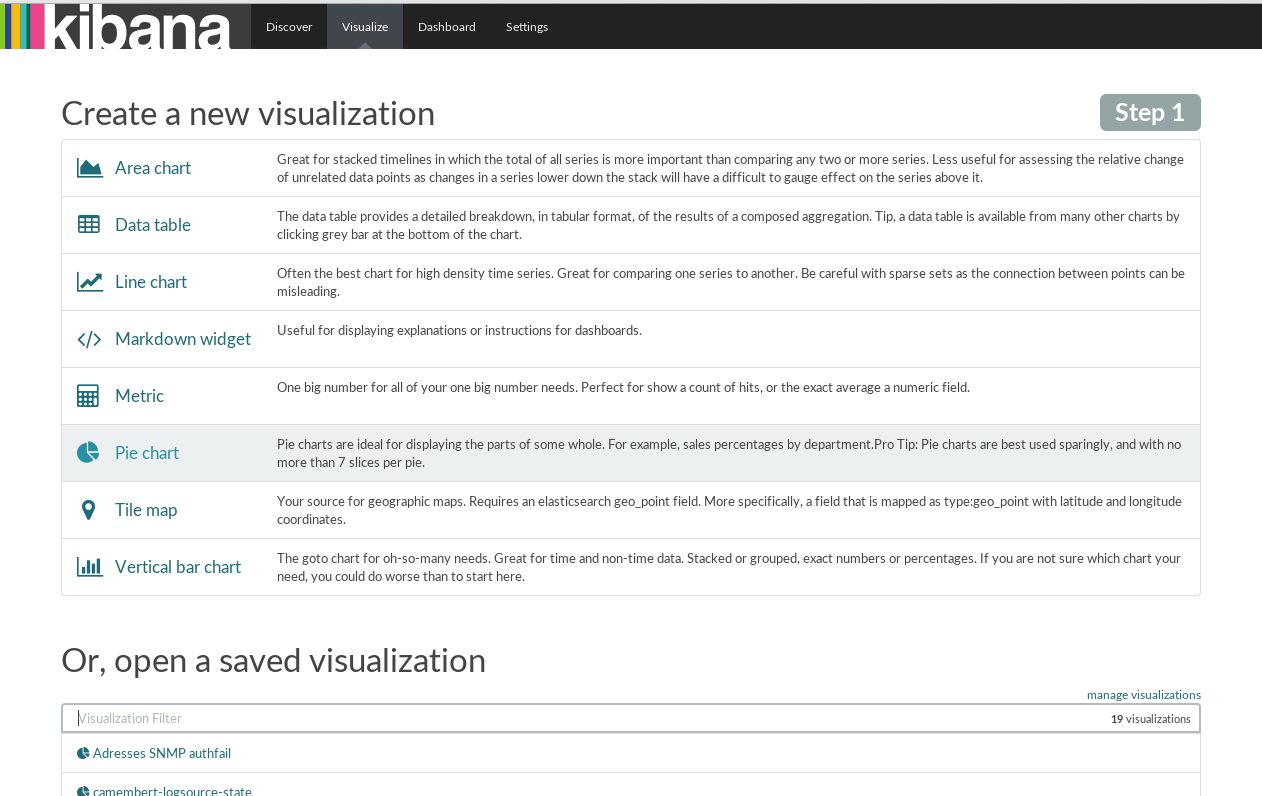
\includegraphics[width=1\textwidth]{kibanatuto/rap/10.png}
\label{fig:kibanatuto7}
\caption{Visualisations possibles}
\end{figure}
Voilà les différents types de visualisations parmi lesquelles nous pouvons faire 
notre choix. Toute ne conviennent pas, le meilleur choix est affaire d'expérience.


\begin{figure}[H]
\center
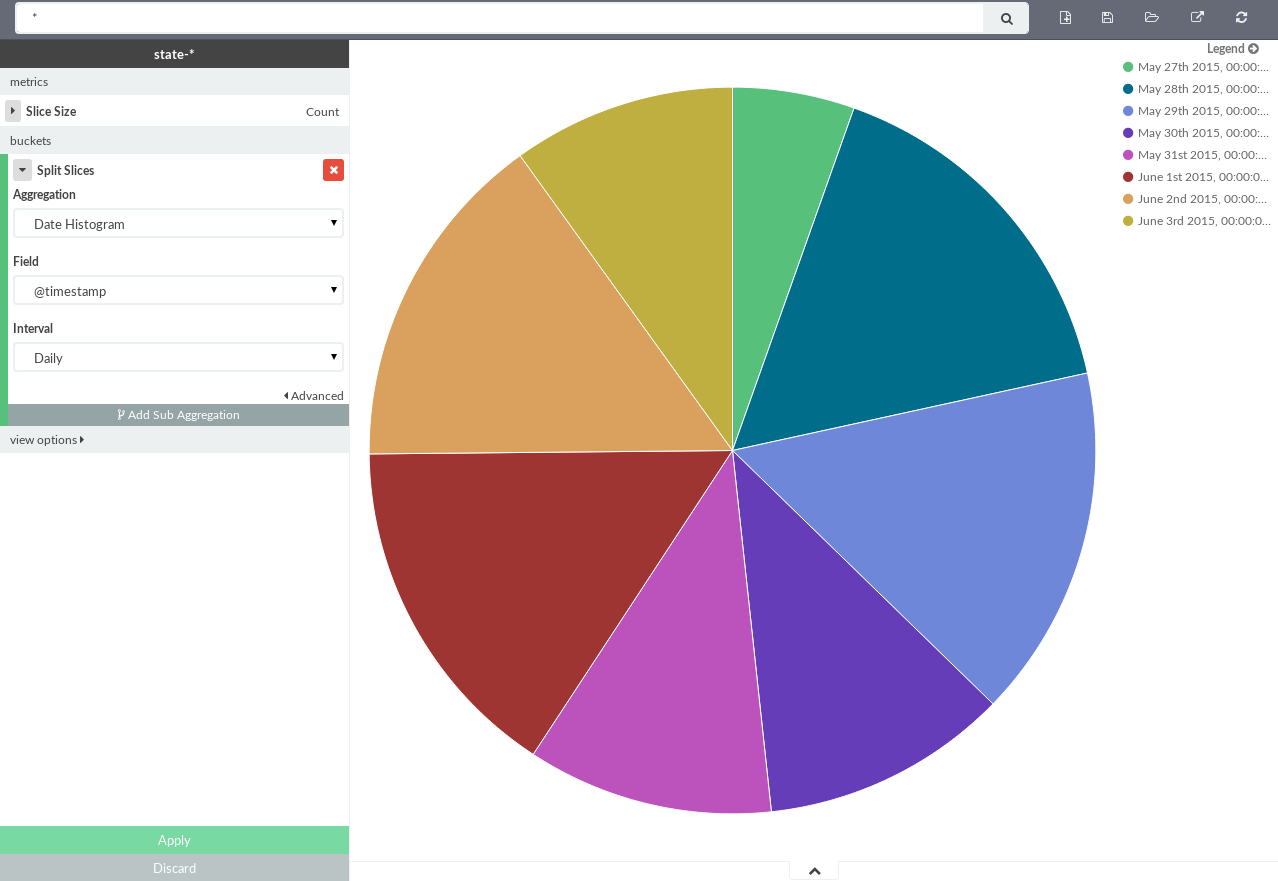
\includegraphics[width=1\textwidth]{kibanatuto/rap/13.png}
\label{fig:kibanatuto8}
\caption{Camembert de répartition des logs sur la dernière semaine}
\end{figure}
Voici un camembert très simple, réalisable en moins d'une minute. Il agrège les logs
sur une semaine en les classants par date d'émission, groupés par jour. 
Il est évidémment possible de faire des choses plus compliquées avec plus ou moins
données/de traitement.


\begin{figure}[H]
\center
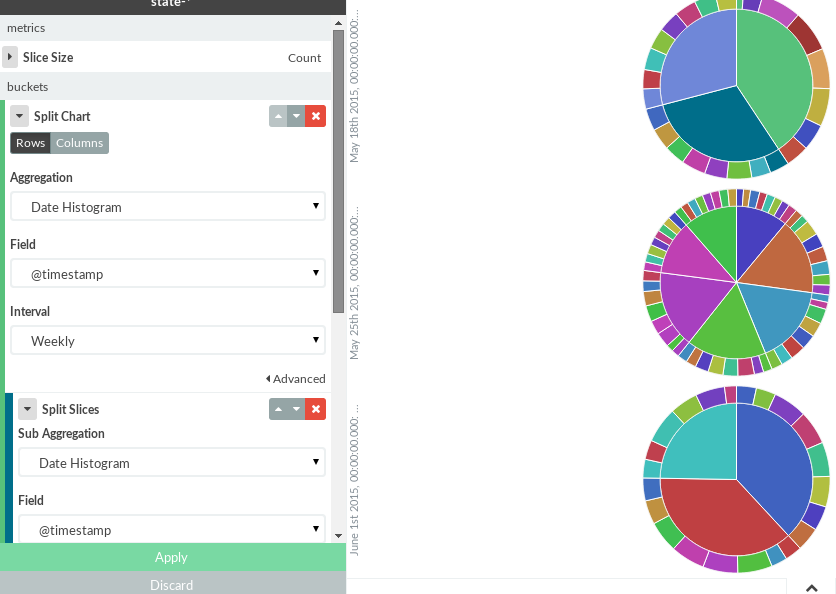
\includegraphics[width=1\textwidth]{kibanatuto/rap/15.png}
\label{fig:kibanatuto9}
\caption{Camembert de répartition des logs sur sur 3 semaines}
\end{figure}
Il s'agit grosso modo des mêmes informations mais cette fois ci groupé par semaine
par camembert, par jour dans le camembert interne, et par tranche de 3h sur l'anneau
externe. Ces camemberts sont interactifs, on le verra dans la partie suivante sur 
les dashboards.


\subsection{Dashboard}
Présentons maintenant les dashboards. Sorte de tableaux virtuels, ils servent à rassembler
les informations. Ces informations ont normalement plus de sens une fois mises cote 
à cote ou permette une analyse plus rapide d'une situation donnée.

La création de ces dashboards est également très simple, on en créer un nouveau en 
appuyant sur le plus à droite.

Il suffit ensuite de choisir les visualisation et ou les recherches enregistrées 
que l'on souhaite voir affiché.

\begin{figure}[H]
\center
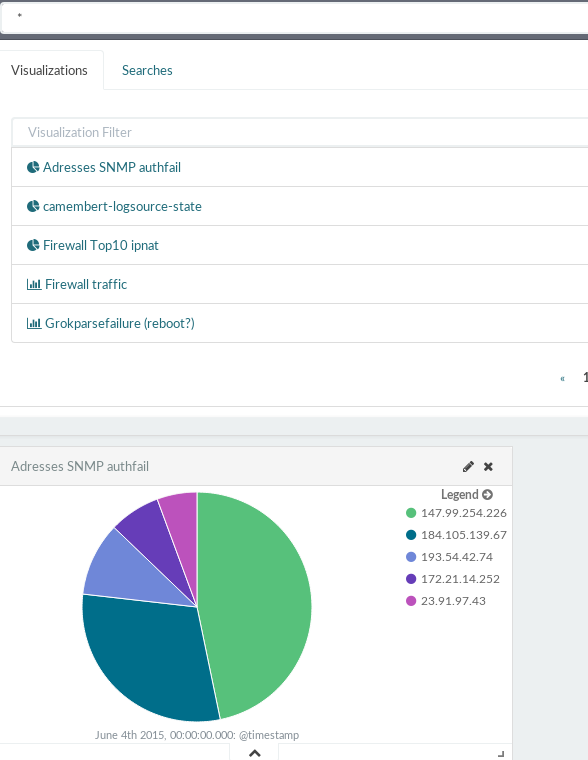
\includegraphics[width=0.8\textwidth]{kibanatuto/rap/17.png}
\label{fig:kibanatuto10}
\caption{Choix des visualisations}
\end{figure}

Comme expliqué plus haut les visualisations ainsi que les tableaux sont interactifs.
Il est par exemple possible de façon assez intuitive faire une recherche limité ségréguée.
Ici il suffit de cliquer sur le quartier désiré de la visualisation. Cela aura pour 
effet de faire apparaitre la barre verte (contextuelle) et de ne faire apparaitre 
dans le tableau de résultat à droite que les logs correspondants. Ici les logs ayant
pour ip source affiché su \hyperref[fig:kibanatuto11]{l'image}.

\begin{figure}[H]
\center
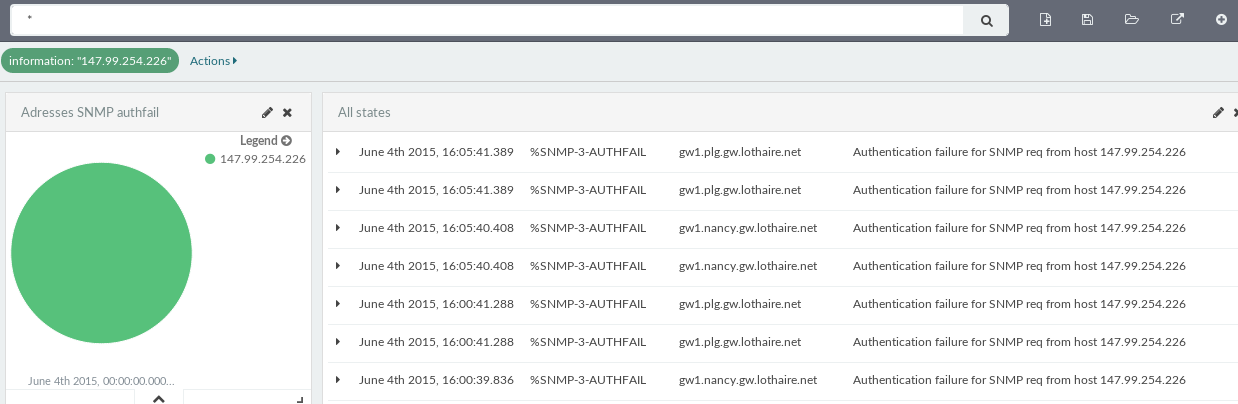
\includegraphics[width=1\textwidth]{kibanatuto/rap/18.png}
\label{fig:kibanatuto11}
\caption{Dashboard simple}
\end{figure}

Il est également possible de facilement partager ces dashboard, via des liens avec 
iframes permettant de les inclure dans une page de monitoring par exemple.

\begin{figure}[H]
\center
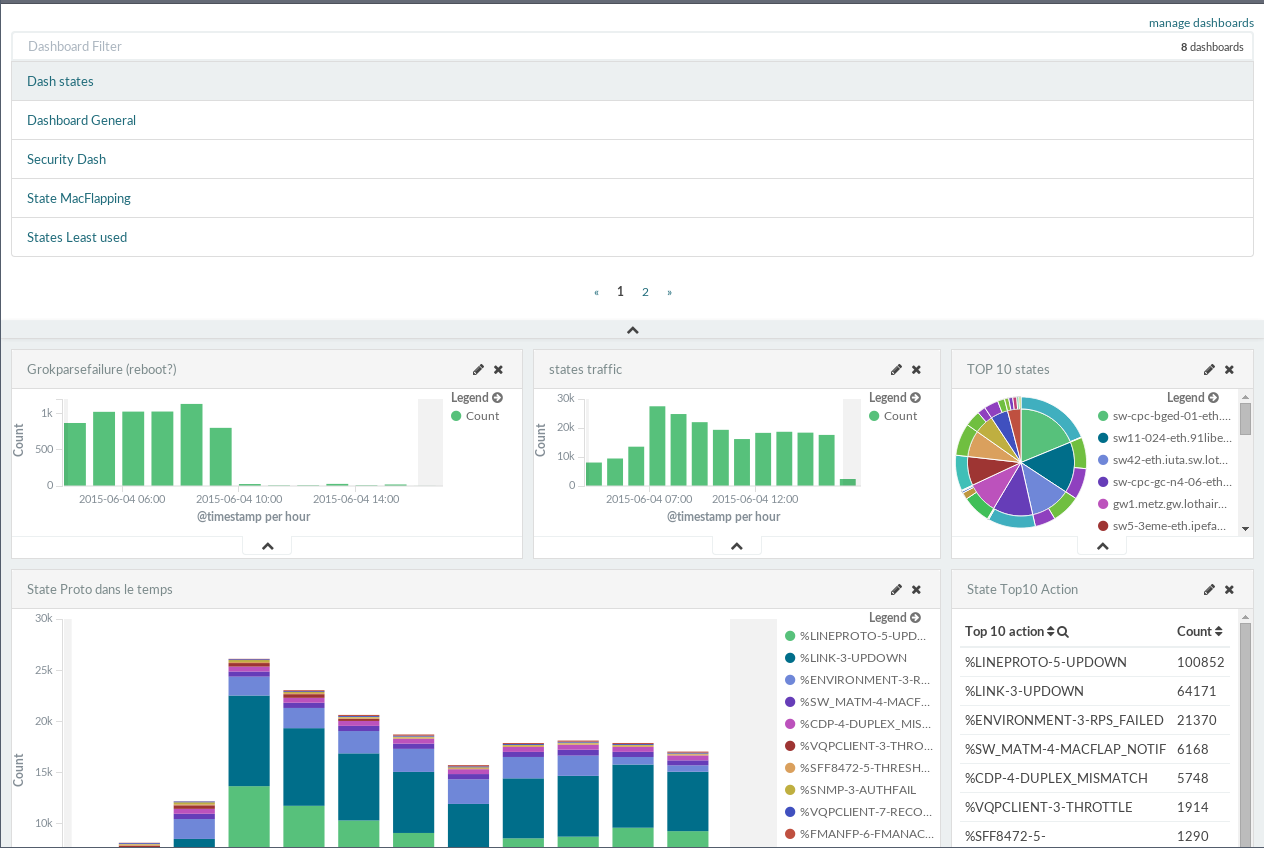
\includegraphics[width=1\textwidth]{kibanatuto/rap/19.png}
\label{fig:kibanatuto12}
\caption{Dashboard plus avancé}
\end{figure}

\subsection{Settings}
Si un doute s'était imissé dans notre esprit, les paramètres de kibana, ne concernent
uniquement kibana, pas Elasticsearch,\hyperref[fig:kibanatuto14]{ certaines informations} 
sont cependant affichées pour aider l'utilisation de kibana mais pas de possibilité 
de les modifiées.

En revanche, il faut bien avouer que leurs consultation est plus agréable depuis 
kibana que depuis l'export json d'Elasticsearch.

\begin{figure}[H]
\center
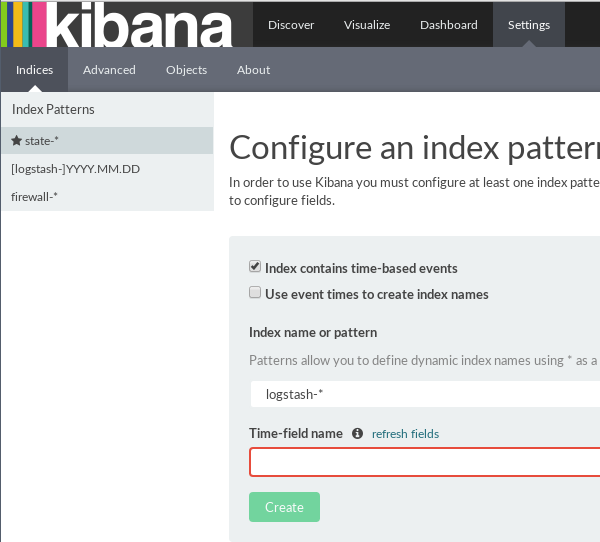
\includegraphics[width=1\textwidth]{kibanatuto/rap/20.png}
\label{fig:kibanatuto13}
\caption{Accueil de settings}
\end{figure}

Dans cette page vous pouvez créer de nouveaux ensembles d'index, ou en choisir un 
déjà existant.

En choisissant un index nous obtenons des informations sur son mapping, ce qui peut 
être utile pour effectué des recherches plus pertinenentes.


\begin{figure}[H]
\center
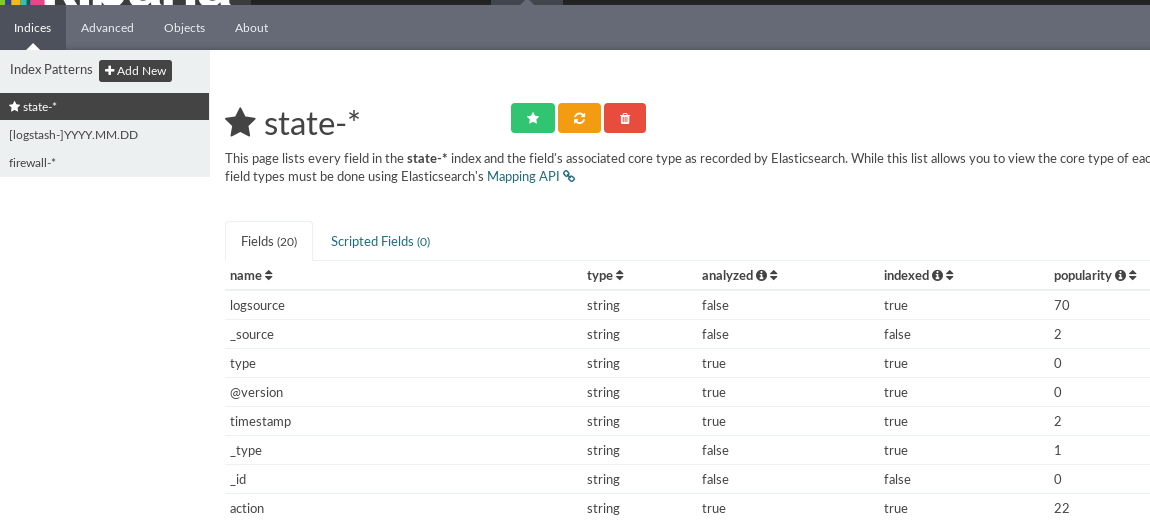
\includegraphics[width=1\textwidth]{kibanatuto/rap/22.png}
\label{fig:kibanatuto14}
\caption{Mapping d'un index}
\end{figure}

Enfin, c'est aussi dans cette section que l'on a une liste et que l'on peut supprimer les 
objets enregistrés (recherche, visualisations, dashboard)

\begin{figure}[H]
\center
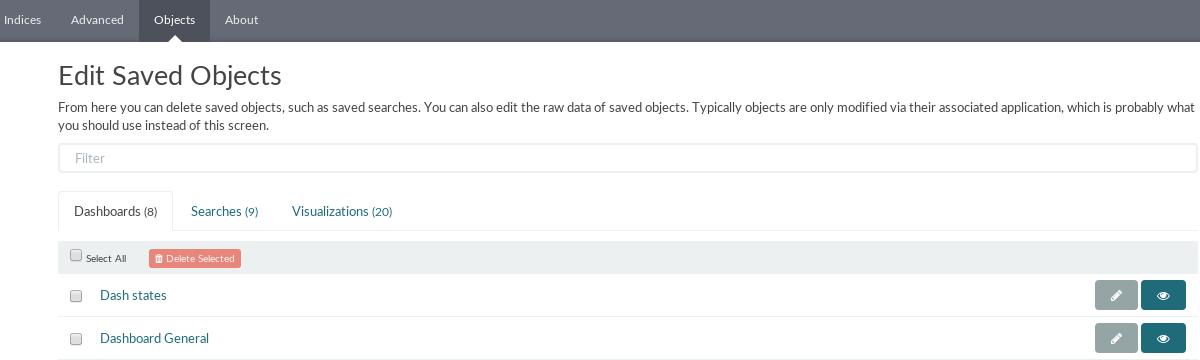
\includegraphics[width=1\textwidth]{kibanatuto/rap/23.png}
\label{fig:kibanatuto15}
\caption{Liste des objets}
\end{figure}

